\subsection{Convolutional Neural Networks}

Convolutional Neural Networks (CNNs) are a specialized class of neural networks designed for processing data with grid-like topology, such as images\cite{LeCun_Bengio_Hinton_2015}.
They are particularly effective for image classification and object detection due to their ability to capture spatial hierarchies in data.
A CNN typically consists of several key layers: convolutional layers, activation layers, pooling layers, and fully connected layers \cite{Venkatesan_Li_2018}.
Let's break down each layer and its role in the network.

\begin{figure}[H]
  % https://vinodsblog.com/2018/10/15/everything-you-need-to-know-about-convolutional-neural-networks/
  \centering
  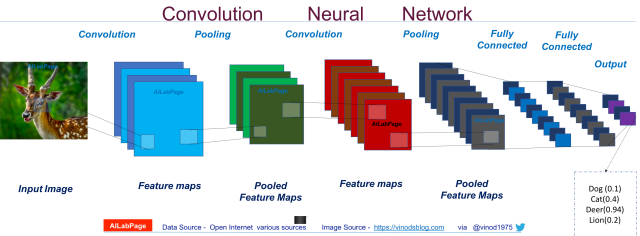
\includegraphics[width=120mm]{figures/cnn.png}
  \caption{Cartoon depicting layers of a CNN\cite{cnn_pic}}
  \label{cnn}
\end{figure}

Convolutional Layer

The convolutional layer is the cornerstone of a CNN.
It applies a set of filters (or kernels) to the input image to produce feature maps \cite{IBM_2024}.
Each filter is a small matrix that slides over the input image to compute a dot product.

Given an input image \( I \) of size \( H \times W \) (height \( H \) and width \( W \)) and a filter \( K \) of size \( k_h \times k_w \) (height \( k_h \) and width \( k_w \)), the output feature map \( O \) can be computed using the convolution operation:

\begin{align}
  O(i, j) &= \sum_{m=0}^{k_h-1} \sum_{n=0}^{k_w-1} I(i+m, j+n) \cdot K(m, n) \\
          &= (I * K)(i, j)
\end{align}

where \( * \) denotes the convolution operation.
The dimensions of the output feature map depend on the stride \( s \) and padding \( p \).
If we use zero-padding and stride \( s = 1 \), the dimensions are:

\begin{align}
  H_{out} &= \frac{H - k_h + 2p}{s} + 1 \\
  W_{out} &= \frac{W - k_w + 2p}{s} + 1
\end{align}

The dimensionality of the output feature map determines how much computational power this step and the following step may take.

Activation Layer 

The Rectified Linear Unit (ReLU) is one of the most commonly used activation functions in CNNs.

This activation function helps in mitigating the vanishing gradient problem and speeds up training.

Pooling Layer

The pooling layer reduces the spatial dimensions of the feature map, which helps in reducing computational complexity and preventing overfitting \cite{Yamaguchi_Sakamoto_Akabane_Fujimoto_1990}.
The most common pooling operation is max pooling.
For a pooling window of size \( p_h \times p_w \) and stride \( s \), the max pooling operation is defined as:

\begin{align}
  O_{pool}(i, j) &= \max_{m \in [i:i+p_h], n \in [j:j+p_w]} O_{ReLU}(m, n)
\end{align}

where \( O_{ReLU} \) is the feature map after applying the ReLU activation.
Pooling reduces the dimensions of the feature map \cite{Ciresan_Meier_Schmidhuber_2012}:

\begin{align}
  H_{out} &= \frac{H - p_h}{s} + 1 \\
  W_{out} &= \frac{W - p_w}{s} + 1
\end{align}

Fully Connected Layer

The fully connected layer (FC layer) is typically used at the end of the network to produce the final classification results.
It connects every neuron in the previous layer to every neuron in the current layer.
The output of a fully connected layer is computed as:

\begin{align}
  z_j &= \sum_{i=1}^{N} w_{ij} x_i + b_j
\end{align}

where \( w_{ij} \) are the weights, \( x_i \) are the inputs from the previous layer, and \( b_j \) is the bias.
This results in a vector of size equal to the number of classes, which can be fed into a softmax function for classification:

\begin{align}
  \text{Softmax}(z_j) &= \frac{e^{z_j}}{\sum_{k} e^{z_k}}
\end{align}

These layers work together to learn hierarchical features from raw data, making CNNs highly effective for various image processing tasks.

